%%%%%%%%%%%%%%%%%%%%%%%%%%%%%%%%%%%%%%%%%
% Article EcoFoG
% Version 2.1 (23/10/2017)
%
% adapté de :
% Stylish Article
% LaTeX Template
% Version 1.0 (31/1/13)
%
% This template has been downloaded from:
% http://www.LaTeXTemplates.com
%
% Original author:
% Mathias Legrand (legrand.mathias@gmail.com)
%
% License:
% CC BY-NC-SA 3.0 (http://creativecommons.org/licenses/by-nc-sa/3.0/)
%
%%%%%%%%%%%%%%%%%%%%%%%%%%%%%%%%%%%%%%%%%


%----------------------------------------------------------------------------------------
%	PACKAGES AND OTHER DOCUMENT CONFIGURATIONS
%----------------------------------------------------------------------------------------

\documentclass[fleqn,10pt]{ArtEcoFoG} % Document font size and equations flushed left

\setcounter{tocdepth}{3} % Show only three levels in the table of contents section: sections, subsections and subsubsections


% Pandoc environments
\usepackage{framed}
\usepackage{fancyvrb}
\providecommand{\tightlist}{%
  \setlength{\itemsep}{0pt}\setlength{\parskip}{0pt}}
\newcommand{\VerbBar}{|}
\newcommand{\VERB}{\Verb[commandchars=\\\{\}]}
\DefineVerbatimEnvironment{Highlighting}{Verbatim}{commandchars=\\\{\}, fontsize=\scriptsize} % Code R
\definecolor{shadecolor}{RGB}{248,248,248}
\newenvironment{Shaded}{\begin{snugshade}}{\end{snugshade}}
\newcommand{\KeywordTok}[1]{\textcolor[rgb]{0.13,0.29,0.53}{\textbf{{#1}}}}
\newcommand{\DataTypeTok}[1]{\textcolor[rgb]{0.13,0.29,0.53}{{#1}}}
\newcommand{\DecValTok}[1]{\textcolor[rgb]{0.00,0.00,0.81}{{#1}}}
\newcommand{\BaseNTok}[1]{\textcolor[rgb]{0.00,0.00,0.81}{{#1}}}
\newcommand{\FloatTok}[1]{\textcolor[rgb]{0.00,0.00,0.81}{{#1}}}
\newcommand{\ConstantTok}[1]{\textcolor[rgb]{0.00,0.00,0.00}{{#1}}}
\newcommand{\CharTok}[1]{\textcolor[rgb]{0.31,0.60,0.02}{{#1}}}
\newcommand{\SpecialCharTok}[1]{\textcolor[rgb]{0.00,0.00,0.00}{{#1}}}
\newcommand{\StringTok}[1]{\textcolor[rgb]{0.31,0.60,0.02}{{#1}}}
\newcommand{\VerbatimStringTok}[1]{\textcolor[rgb]{0.31,0.60,0.02}{{#1}}}
\newcommand{\SpecialStringTok}[1]{\textcolor[rgb]{0.31,0.60,0.02}{{#1}}}
\newcommand{\ImportTok}[1]{{#1}}
\newcommand{\CommentTok}[1]{\textcolor[rgb]{0.56,0.35,0.01}{\textit{{#1}}}}
\newcommand{\DocumentationTok}[1]{\textcolor[rgb]{0.56,0.35,0.01}{\textbf{\textit{{#1}}}}}
\newcommand{\AnnotationTok}[1]{\textcolor[rgb]{0.56,0.35,0.01}{\textbf{\textit{{#1}}}}}
\newcommand{\CommentVarTok}[1]{\textcolor[rgb]{0.56,0.35,0.01}{\textbf{\textit{{#1}}}}}
\newcommand{\OtherTok}[1]{\textcolor[rgb]{0.56,0.35,0.01}{{#1}}}
\newcommand{\FunctionTok}[1]{\textcolor[rgb]{0.00,0.00,0.00}{{#1}}}
\newcommand{\VariableTok}[1]{\textcolor[rgb]{0.00,0.00,0.00}{{#1}}}
\newcommand{\ControlFlowTok}[1]{\textcolor[rgb]{0.13,0.29,0.53}{\textbf{{#1}}}}
\newcommand{\OperatorTok}[1]{\textcolor[rgb]{0.81,0.36,0.00}{\textbf{{#1}}}}
\newcommand{\BuiltInTok}[1]{{#1}}
\newcommand{\ExtensionTok}[1]{{#1}}
\newcommand{\PreprocessorTok}[1]{\textcolor[rgb]{0.56,0.35,0.01}{\textit{{#1}}}}
\newcommand{\AttributeTok}[1]{\textcolor[rgb]{0.77,0.63,0.00}{{#1}}}
\newcommand{\RegionMarkerTok}[1]{{#1}}
\newcommand{\InformationTok}[1]{\textcolor[rgb]{0.56,0.35,0.01}{\textbf{\textit{{#1}}}}}
\newcommand{\WarningTok}[1]{\textcolor[rgb]{0.56,0.35,0.01}{\textbf{\textit{{#1}}}}}
\newcommand{\AlertTok}[1]{\textcolor[rgb]{0.94,0.16,0.16}{{#1}}}
\newcommand{\ErrorTok}[1]{\textcolor[rgb]{0.64,0.00,0.00}{\textbf{{#1}}}}
\newcommand{\NormalTok}[1]{{#1}}
\usepackage{longtable,booktabs}
\usepackage{caption}
% These lines are needed to make table captions work with longtable:
\makeatletter
\def\fnum@table{\tablename~\thetable}
\makeatother
% longtable 2 columns
% https://tex.stackexchange.com/questions/161431/how-to-solve-longtable-is-not-in-1-column-mode-error
\makeatletter
\let\oldlt\longtable
\let\endoldlt\endlongtable
\def\longtable{\@ifnextchar[\longtable@i \longtable@ii}
\def\longtable@i[#1]{\begin{figure}[t]
\onecolumn
\begin{minipage}{0.5\textwidth}\scriptsize
\oldlt[#1]
}
\def\longtable@ii{\begin{figure}[t]
\onecolumn
\begin{minipage}{0.5\textwidth}\scriptsize
\oldlt
}
\def\endlongtable{\endoldlt
\end{minipage}
\twocolumn
\end{figure}}
\makeatother

\usepackage{graphicx,grffile}
\makeatletter
\def\maxwidth{\ifdim\Gin@nat@width>\linewidth\linewidth\else\Gin@nat@width\fi}
\def\maxheight{\ifdim\Gin@nat@height>\textheight0.8\textheight\else\Gin@nat@height\fi}
\makeatother
% Scale images if necessary, so that they will not overflow the page
% margins by default, and it is still possible to overwrite the defaults
% using explicit options in \includegraphics[width, height, ...]{}
\setkeys{Gin}{width=\maxwidth,height=\maxheight,keepaspectratio}

% User-adder preamble
\usepackage{textcomp} \DeclareUnicodeCharacter{B0}{\textdegree}
\usepackage{tabu}
\renewenvironment{table}{\begin{table*}}{\end{table*}\ignorespacesafterend}
\hyphenation{bio-di-ver-si-ty sap-lings}

%----------------------------------------------------------------------------------------
%	ARTICLE INFORMATION
%----------------------------------------------------------------------------------------

\JournalInfo{Hal xxx} % Journal information
\Archive{DOI xxxx} % Additional notes (e.g. copyright, DOI, review/research article)

\PaperTitle{Post-Disturbance Tree Community Trajectories in a Neotropical Forest} % Article title

\Authors{
Ariane MIRABEL\textsuperscript{1*}\\ Eric Marcon\textsuperscript{1}\\ Bruno Hérault\textsuperscript{2 3}
} % Authors
\affiliation{
\textsuperscript{1}UMR EcoFoG, AgroParistech, CNRS, Cirad, INRA, Université des Antilles,
Université de Guyane.\\ \hspace{1em} Campus Agronomique, 97310 Kourou, France.\\\textsuperscript{2}Cirad, Univ montpellier, UR Forests \& Societies.\\ \hspace{1em} Montpellier, France.\\\textsuperscript{3}INPHB, Institut National Polytechnique Félix Houphouet-Boigny\\ \hspace{1em} Yamoussoukro, Ivory Coast.
}
\affiliation{*\textbf{Corresponding author}: ariane.mirabel@ecofog.gf, http://www.ecofog.gf/spip.php?article47} % Corresponding author

\Keywords{mot-clés, séparés par des virgules} % Keywords - if you don't want any simply remove all the text between the curly brackets
\newcommand{\keywordname}{Keywords} % Defines the keywords heading name

%----------------------------------------------------------------------------------------
%	ABSTRACT
%----------------------------------------------------------------------------------------

\Abstract{
Résumé de l'article.
}

%----------------------------------------------------------------------------------------

\usepackage{amsthm}
\newtheorem{theorem}{Theorem}[section]
\newtheorem{lemma}{Lemma}[section]
\theoremstyle{definition}
\newtheorem{definition}{Definition}[section]
\newtheorem{corollary}{Corollary}[section]
\newtheorem{proposition}{Proposition}[section]
\theoremstyle{definition}
\newtheorem{example}{Example}[section]
\theoremstyle{definition}
\newtheorem{exercise}{Exercise}[section]
\theoremstyle{remark}
\newtheorem*{remark}{Remark}
\newtheorem*{solution}{Solution}
\begin{document}

\selectlanguage{english}

\flushbottom % Makes all text pages the same height

\maketitle % Print the title and abstract box

\tableofcontents % Print the contents section

\thispagestyle{empty} % Removes page numbering from the first page

%----------------------------------------------------------------------------------------
%	ARTICLE CONTENTS
%----------------------------------------------------------------------------------------






















\section{Introduction}\label{introduction}

The large areas covered with tropical forests worldwide hold crucial
economic, social and cultural value. They provide wood and multiple
non-timber forest products, shelter for a diversified fauna, regulate
the local climate, support the carbon, water and nutrient cycles, and
ensure cultural and human well-being. The simultaneous increase of
forests products demand and substantial climatic changes heightened the
pressure on the remaining forests
\citep{Gibson2011a, Morales-Hidalgo2015} and threatened the maintenance
of communities structure, composition and functioning and their
underlying dynamics \citep{Anderson-Teixeira2013, Sist2015}.

In tropical forests communities are shaped by a constant range of
disturbance that changes the abiotic environment, as the light, heat and
water fluxes, and the biotic interaction and competitive pressure. The
cornerstone of tropical forests ecology is then to understand their
response to disturbance and the corresponding mechanisms
\citep{White2001, Chazdon2003a}. Forests response to disturbance has
been largely studied through structural parameters rapid and convenient
to measure, as aboveground biomass, tree height or stem density. These
structural parameters have then been sucessfully modeled and assessed
the maintenance of ecosystems processes and services
\citep{Denslow2000, Blanc2009, Rutishauser2016}. However the response of
tree species diversity although it is determinant of ecosystems
productivity, stability and functioning \citep{Tilman2014} and it would
be most probably impacted by the biotic and abiotic changes after
disturbance \citep{CazzollaGatti2014}.

In the short-term, diversity dynamics demonstrated negligible or even
positive impacts of disturbance on communities diversity, and have been
formalized by the intermediate disturbance hypothesis (IDH) that
predicts a maximized species diversity at intermediate level of
disturbance\citep{Molino2001, Kariuki2006a, Berry2008a}. The IDH however
has scarcely been tested in the long term and mainly relied on the
analysis of species richness that gives limited or misleading
information on forests recovery and functioning
\citep{Martin2015, Chaudhary2016}. Communities composition and evenness
are crucial to resolve conservation issues and assess the ecological
rules shaping communities abundance distribution
\citep{Magurran1988, Lavorel2002, Bellwood2006}. A promosing perspective
is also the functional approach accounting for species biological
attributes related to individuals fitness and ecosystem properties
\citep{Violle2007b, Moretti2009, Baraloto2012a, Scheiter2013}. Major
functional traits revealing species ecology and performance were largely
adopted through a workable framework assessing forests dynamics and
functioning \citep{Diaz2005, Villeger2008a}. This approach for example
highlighted in tropical rainforests the environmental filters fostering
disturbance resistant species with rapid growth and efficient resources
acquisition \citep{Molino2001, Haddad2008}. This was translated by the
shift from ``conservative'' species with long-lived, dense tissues
growing slowly but with scarce resources, to ``acquisitive''
fast-growing species with light tissues and efficient resources use
\citep{TerSteege2001, Reich2014, Herault2011}. Such shift would be
detected with a combination of resource acquisition funcitonal traits
(leaf area, density and chlorophyll content and stem specific gravity
and bark thickness) and growth and reproduction life history traits
(seed mass and maximum height) already proved relevant
\citep{Wright2004, Westoby2006a, Chave2009b}. A functional approach
combined to the analysis of taxonomic diversity and composition is then
a reliable way to validate the IDH in the long term and from communities
evenness and functinal perspective. A full interpretation of communities
response would be completed with communities taxonomic and functional
composition that would elucidate the determinism of forest recovery and
the maintenance of intrinsinc differences. Those development would be as
much information to understand the mechanisms of forests response to
diversity and help conservation and management strategies.

Here we investigated over 30 years the response of 75 ha of forests
plots set up on a gradient of disturbance intensity, from 10 to 60\% of
ecosystem biomass removed. We made use of a large functional traits
database browsing major leaf, stem and seed traits and species maximum
height to draw communities taxonomic and functional composition and
diversity trajectories after disturbance. Specifically, we (i) tested
the validity of the IDH arguing for enhanced diversity after moderate
disturbance and (ii) confirmed the changes in ecological rules shaping
communities, from competitive exclusion between ``conservative'',
slow-growing tree species to environmental filtering of ``acquisitive'',
fasting-growing ones. Eventually we examined the different trajectories
to (iii) resolve the resilience of tropical forests and question their
future dynamics regarding their state 30 years after disturbance.

\section{Material and Methods}\label{material-and-methods}

\subsection{Study site}\label{study-site}

Paracou station in French Guiana (5°18'N and 52°53'W) is located in a
lowland tropical rain forest corresponding to a tropical wet climate
with mean annual precipitation averaging 2980 mm.y\textsuperscript{-1}
(30-y period) with a 3-months dry season (\textless{} 100
mm.months\textsuperscript{-1}) from mid-August to mid-November, and a
one-month dry season in March \citep{Wagner2011}. Elevation ranges
between 5 and 50 m and mean annual temperature is 26°C. Soils correspond
to thin acrisols over a layer of transformed saprolite with low
permeability generating lateral drainage during heavy rains. The
experiment corresponds to a network of twelve 6.25ha plots that have
undergone a gradient of three logging, thinning and fuelwood treatments
(Table \ref{tab:Tab1}). Disturbance treatments were attributed according
to a randomized plot design with three replicate blocks of four plots.
The disturbance corresponds to averages of 10 trees removed per hectare
with a diameter at 1.3 m height (DBH) above 50 cm for treatment 1 (T1),
32 trees/ha above 40 cm DBH for treatment 2 (T2) and 40 trees above 40
cm DBH for treatment 3 (T3). Treatments T2 and T3 besides included the
thinning of trees by poison girdling \citep{Blanc2009}.

\begin{table}

\caption{\label{tab:Tab1}Intervention table, summary of the disturbance intensity for the 4 plot treatments in Paracou.}
\centering
\begin{tabu} to \linewidth {>{\raggedright}X>{\raggedright}X>{\raggedright}X>{\raggedright}X>{\raggedright}X}
\toprule
Treatment & Timber & Thinning & Fuelwood & \%AGB lost\\
\midrule
Control &  &  &  & 0\\
T1 & DBH $\geq$ 50 cm, commercial species, $\approx$ 10 trees/ha &  &  & $[12\%-33\%]$\\
T2 & DBH $\geq$ 50 cm, commercial species, $\approx$ 10 trees/ha & DBH $\geq$ 40 cm, non-valuable species, $\approx$ 30 trees/ha &  & $[33\%-56\%]$\\
T3 & DBH $\geq$ 50 cm, commercial species, $\approx$ 10 trees/ha & DBH $\geq$ 50 cm, non-valuable species, $\approx$ 15 trees/ha & 40 cm $\leq$ DBH $\leq$ 50 cm, non-valuable species, $\approx$ 15 trees/ha & $[35\%-56\%]$\\
\bottomrule
\end{tabu}
\end{table}

\subsection{Inventories protocol and dataset
collection}\label{inventories-protocol-and-dataset-collection}

The study site corresponds to a tropical rainforest with a dominance of
Fabaceae, Chrysobalanaceae, Lecythidaceae and Sapotaceae botanical
families. In the twelve experimental plots of the experiment, all trees
above 10 cm DBH were mapped and measured annually since 1984. During
inventories, trees were first identified with a vernacular name assigned
by the field team, and afterward with a scientific name assigned by a
botanist during regular botanical campaigns. In 1984, specific
vernacular names were given to 62 commercial or common species whereas
other less common species were identified under two identifiers only
separating trees and palm trees. The botanical campaigns carried every 5
to 6 years to identify all trees at the species level only started in
2003 and identification practices varied among plots and successive
campaigns. This raised methodological issues as vernacular names usually
correspond to different botanical species, resulting in significant
taxonomic uncertainties that had to be propagated to composition and
diversity metrics throught a Bayesian framework. The uncertainty
propagation was done by the replenishment of inventories completed at
genus level from real incomplete ones on the basisof
vernacular/botanical names association.

Vernacular names were replaced through multinomial trials
\(M_v\Big(\big[s_1, s_2, …, s_N\big],\big[\alpha_1, \alpha_2,…, \alpha_3\big]\Big)\)
based on the observed association probability
\(\big[\alpha_1, \alpha_2,…, \alpha_3\big]\) between each vernacular
name \emph{v} and the species \(\big[s_1, s_2, …, s_N\big]\) recorded in
the inventory.

To avoid remaining identification caveats and consider complete
inventories, the simulated inventories were then reported at genus. See
appendix 1 and \citet{Aubry-Kientz2013} for the detailed methodology.

The functional diversity metrics used a dataset for 6 functional traits
representing leaf economics (leaves thickness, toughness, total
chlorophyll content and specific leaf area, the leaf area per unit dry
mass) and wood economics (wood specific gravity and bark thickness), and
life history traits (maximum specific height and seed mass).

The trait database came from the BRIDGE project {[}\^{}1{]} where traits
values were assessed from a selection of individuals located in nine
permanent plots in French Guiana, including two in Paracou. Missing
trait values were filled using multivariate imputation by chained
equation (mice) restricted to samples pertaining to the next higher
taxonomic level, in order to account for the phylogenetic signal of the
functional traits. The dataset comprised 294 botanical species
pertaining to 157 botanical genera.

Whenever a species inventoried was not in the dataset, it was attributed
a set of traits values randomly sampled among species of the same next
higher taxonomic level. As seed mass information corresponds to a
classification into mass classes, no data filling process was applied so
analysis were performed considering the 414 botanical species of the
seed mass dataset. All composition and diversity metrics corresponded to
the average obtained after 50 iterations of the taxonomic uncertainty
propagation framework and of the filling process of missing trait
values.

{[}\^{}1{]} http://www.ecofog.gf/Bridge/

\subsection{Composition and diversity
metrics}\label{composition-and-diversity-metrics}

To counter the remaining taxonomic uncertainty plots taxonomic
composition and diversity were analysed at the genus level, \emph{i.e.}
referring to the genus of observed or trialed botanical names. The
analysis of taxonomic and functional composition of plots along time was
visualized in a two-dimensional ordination space based on non-metric
dimensional scaling of succesive floristic or functional inventories.
Plots trajectories along time was reported comparatively to the
inventories in 1989, 5 years after disturbance, which corresponded to
first inventory with a sufficient degree of uncertainty (\textless{}30\%
of undetermined trees). The inventories dissimilarity compared to the
reference 1989 inventory was reported using occurrence-based (Jaccard)
and abundance-based (Bray-Curtis) similarity measures. The trajectory of
inventories along time was visualized with the euclidean distance in the
two-dimensional ordination space to the 1989 inventory. The functional
trajectories of the leaf and stem and life traits were also visualized
with the community weighted means (CWM), representing the average trait
value in a community weighted by relative abundance of the species
carrying each value \citep{Diaz2007, Garnier2004}. Species seed mass
corresponded to 5 classes of increasing mass, seed mass trajectories
were therefore reported as the proportion of each class in the
inventories.

The taxonomic diversity was assessed through Richness and the Hill
number translation of Shannon and Simpson indices \citep{Hill1973}.
\textgreater{}\textgreater{}To tackle the unequal number of recruited
trees among treatments the indices bias corrected estimator were used,
following \citep{Chao2015, Marcon2015b}.

These three indices belong to the set of HCDT or generalized entropy,
respectively corresponding to the 0, 1 and 2 order of diversity (q),
which proved well suited for diversity studies
\citep{Patil1982, Tothmeresz1995}. The functional diversity was reported
using the Rao index of quadratic entropy which combines species
abundance distribution and average pairwise dissimilarity based on all
functional and life traits.

\section{Results}\label{results}

\subsection{Taxonomic and functional
composition}\label{taxonomic-and-functional-composition}

\subsubsection{Composition trajectories}\label{composition-trajectories}

Over time, 828388 trees and 591 botanical species pertaining to 223
genus and 64 botanical families were recorded. Trajectories of taxonomic
and functional composition after disturbance were examined through the
ordination of successive inventories from 1989 (5 years after
disturbance) in the two-dimensional space from NMDS analysis based on
flora inventories and the corresponding functional composition.
Classifications were performed using either abundance-based Bray-Curtis
(Figure \ref{fig:NMDSplans}) or incidence-based Jaccard dissimilarity
(data not shown).

Both taxonomic and functional composition were substantially affected by
disturbance, and the maximum dissimilarity to 1984 reference inventory
composition was positively correlated with the disturbance intensity.
Until 30 years after disturbance, all disturbed plots taxonomic
composition remained significantly dissimilar to that of the 1989
reference inventory composition (Figure \ref{fig:NMDSplans}). All plots,
though, displayed a unimodal trajectory with a the return toward the
taxonomic and functional composition of the 1989 reference inventory
suggesting a shift towards a cyclic regime (Figure
\ref{fig:NMDSdivergence}). For taxonomic composition, the maximum
dissimilarity to 1984 inventory composition was reach around 20 years
after disturbance for the T2 and T3 plots and for one T1 plot while
control and other T1 plots continued to increase (Figure
\ref{fig:NMDSdivergence}.a). For functional composition, the maximum
dissimilarity to 1984 inventory composition was reach from 15 to 20
years after disturbance for the T2 and T3 plots while T1 and control
plots continued to increase (Figure \ref{fig:NMDSdivergence}.b). The
functional composition distancing from the reference inventory was also
positively correlated with disturbance intensity and similarly
stabilized or reduced (for 5 of T1, T2 and T3 plots) from 20 years after
disturbance (Figure \ref{fig:NMDSdivergence}).

The coordinates of the functional traits were measured in the
two-dimensional ordination space that mapped plots evolution along time
(graphs not showed) revealed a trajectory of disturbed plots toward
acquisitive functional strategies (from high WD to high SLA and
chlorophyll content).

\begin{figure*}

{\centering 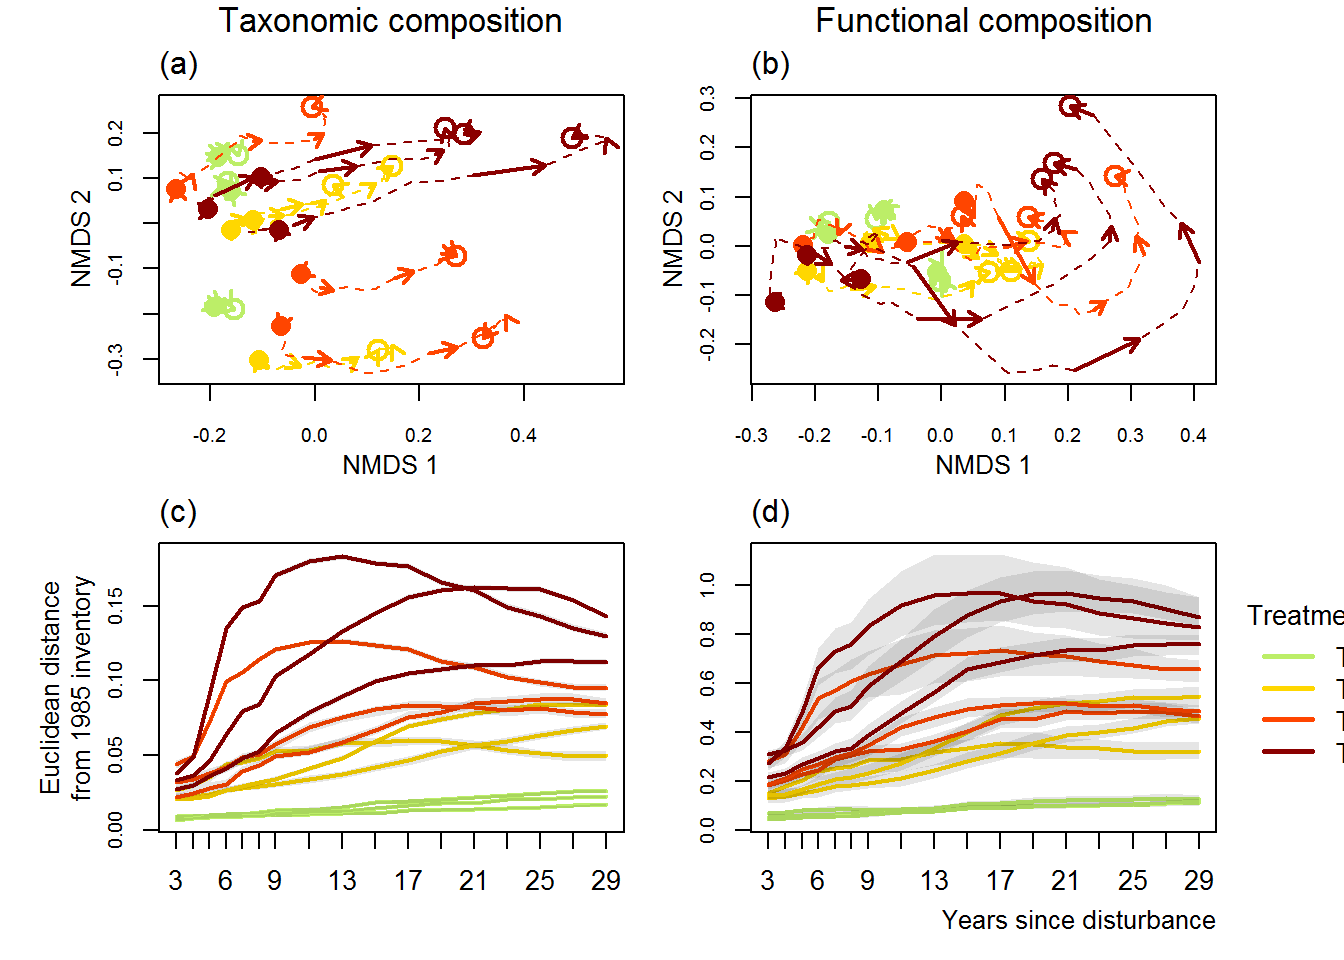
\includegraphics[width=1\linewidth]{WholePlotTrajectories_files/figure-latex/NMDSplans-1} 

}

\caption{Trajectories of the plots in terms of \textbf{(a)} flora composition and \textbf{(b)} functional composition regarding the 6 leaf and stem functional traits,the maximum allometric height and seed mass class in the two-dimensional space from the NMDS performed for the 30 years after disturbance. Distance matrix for NMDS were computed from the Bray-curtis dissimilarity between successive inventories. Line colors represent the disturbance treatment (green for control, blue for T1,orange for T2 and red for T3).}\label{fig:NMDSplans}
\end{figure*}

\begin{figure}

{\centering 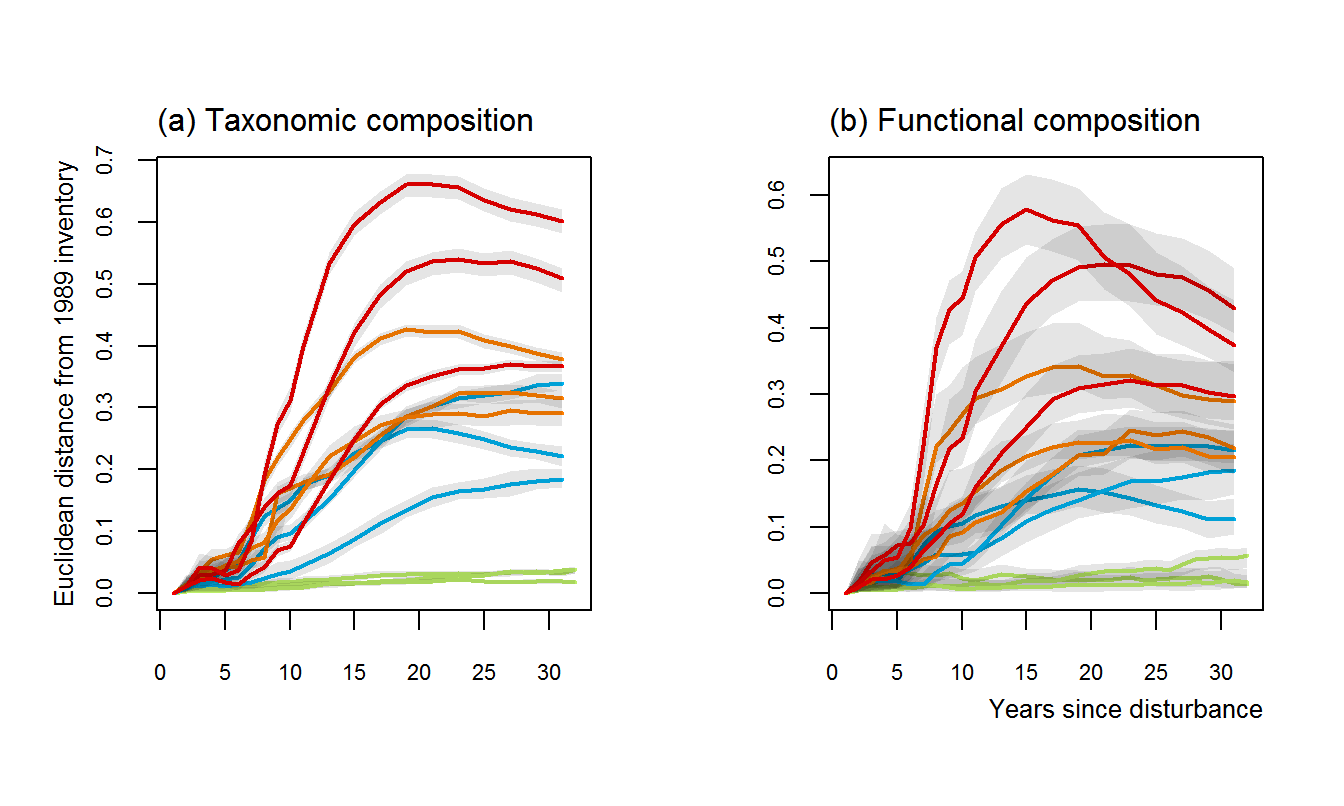
\includegraphics[width=1\linewidth]{WholePlotTrajectories_files/figure-latex/NMDSdivergence-1} 

}

\caption{Trajectories of the distance to initial condition of the 30 sampled years in the two-dimensional space from the NMDS of v taxonomic composition at genus level and \textbf{(b)} functional composition. Distance are abundance-based Bary-Curtis metric. Line colors represent the disturbance treatment (green for control, blue for T1,orange for T2 and red for T3). The 0.025 and 0.975 percentile correspond to the variance observed for 50 iteration of the taxonomic uncertainty propagation and functional trait filling processes. }\label{fig:NMDSdivergence}
\end{figure}

\subsubsection{Traits community weighted
means}\label{traits-community-weighted-means}

For all plots the trajectories of the community weighted means (CWM)
were drawn for the 8 functional and life history traits (Leaf thickness,
chlorophyll content, toughness and specific area,wood specific gravity
and barck thickness and seed mass and maximum adult height) (Figure
\ref{fig:CWM}).

To compensate the intrinsinc difference among plots the trajectories
drawn correspond to the difference in value between the reference
inventory in 1984 (5 year after disturbance) and the successive years
inventoried.

Except for leaf cholorphyll content, which displayed higher difference
between plots than among treatments which may be due to the completeness
of dataset, all CWM trajectories corresponded to significant changes
after disturbance. All functional traits and seed mass proportions
displayed a unimodal trajectories but with different times at maximum
and different values 30 years after disturbance. The weighted means of
communities specific maximum height at adult stage (\emph{Hmax}), leaf
toughness (\emph{L\_toughness}) and wood specific gravity (\emph{WD})
remained significantly lower than their initial value and than these of
the control plots (Figure \ref{fig:CWM}). The weighted means of bark
thickness (\emph{Bark\_thick}) similarly remained substantilly higher
than initially for all disturbed plots while the specfic leaf area
(\emph{SLA}) had almost recovered its initial value and this of the
undisturbed plots at the end of the experiment.

\begin{figure*}

{\centering 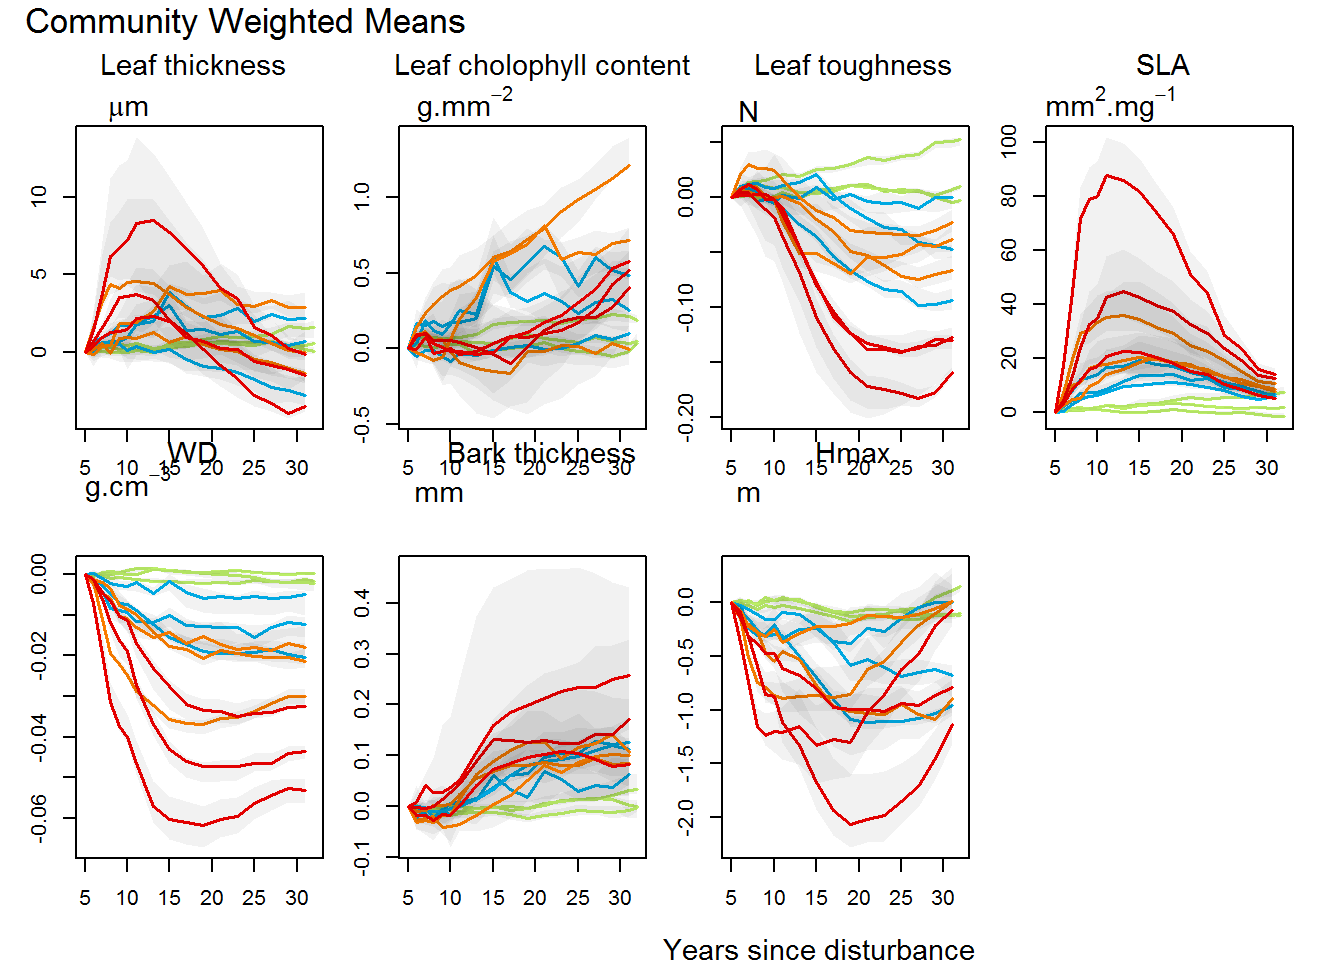
\includegraphics[width=1\linewidth]{WholePlotTrajectories_files/figure-latex/CWM-1} 

}

\caption{Trajectories of the communities weighted means (CWM) over 30 years after disturbance of 4 leaf traits (Leaf thickness, \emph{L\_thickness}, chlorophyll content, \emph{L\_chloro}, toughness, \emph{L\_toughness} and specific area, \emph{SLA}), 2 stem traits (wood specific gravity, \emph{WD}, and bark thickness, \emph{Bark-thick}) and one life trait (Specific maximum height at adult stage, \emph{Hmax}). Trajectories correspond to the median (solid line) and 0.025 and 0.975 percentile (gray envelope) observed after 50 iteration of the taxonomic uncertainty propagation and the missing trait value filling processes. Initial treatments are represented by solid lines colorswith green for control, blue for T1,orange for T2 and red for T3.}\label{fig:CWM}
\end{figure*}

\subsection{Disturbance impact on
diversity}\label{disturbance-impact-on-diversity}

\subsubsection{Taxonomic diversity}\label{taxonomic-diversity}

Trajectories of Richness, Shannon and Simpson taxonomic diversity were
examined at genus level in relation to the 1989 inventories (5 years
after disturbance) (Figure \ref{fig:DivTaxo}).

\begin{figure*}

{\centering 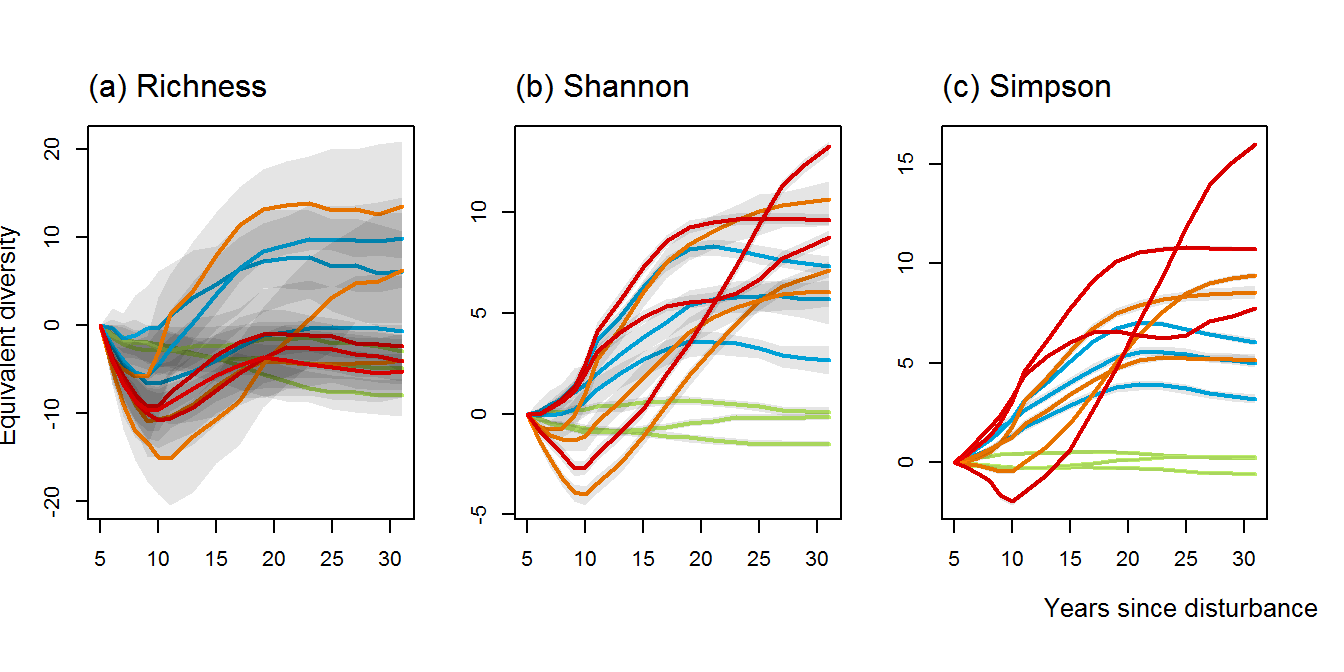
\includegraphics[width=1\linewidth]{WholePlotTrajectories_files/figure-latex/DivTaxo-1} 

}

\caption{Trajectories of the difference to the 1989 inventories (5 years after disturbance) over 30 years after disturbance of plots communities \textbf{(a)} Richness, \textbf{(b)} Shannon and \textbf{(c)} Simpson diversities. Trajectories correspond to the median (solid line) and 0.025 and 0.975 percentile (gray envelope) observed after 50 iteration of the taxonomic uncertainty propagation. Initial treatments are represented by solid lines colors with green for control, blue for T1,orange for T2 and red for T3.}\label{fig:DivTaxo}
\end{figure*}

For undisturbed plots the Richness, Shannon and Simpson diversity
remained comparable to the initial values 5 years after disturbance.
After disturbance, the richness increased after low disturbance
intensity, with a maximum increase of 14 botanical genuses (for plot 3
after treatment 2), but followed a unimodal decrease with a return to
initial values after intense disturbance. The taxonomic evenness
(Shannon and Simpson diversities), however, significantly increased
after all disturbance regime. The evenness followed a unimodal
trajectory with a just beginning return towards initial values and a
maximum reached around 20 years and positively correlated to the
disturbance intensity (\(\rho_{spearman}^{Shannon}=0.92\), and
\(\rho_{spearman}^{Simpson}=0.97\)). Only two T3 plots, plots 8 and 12,
remained increasing 30 years after disturbance \ref{fig:DivTaxo}),
suggesting a similar be much delayed unimodal trajectory.

\subsubsection{Functional diversity}\label{functional-diversity}

For all undisturbed plots the Rao diversity remained comparable to the
initial values, 5 years after disturbance (1989 inventories). The
trajectories of all disturbed plots followed a unimodal trajectory with
a maximum positively correlated to disturbance intensity
(\(\rho_{spearman}\)) (Figure \ref{fig:DivFun}). Thirty years after
disturbance all plots, whenever the initial disturbance intensity,
regained diversity values similar to their initial avule and to those of
control plots.

\begin{figure}

{\centering 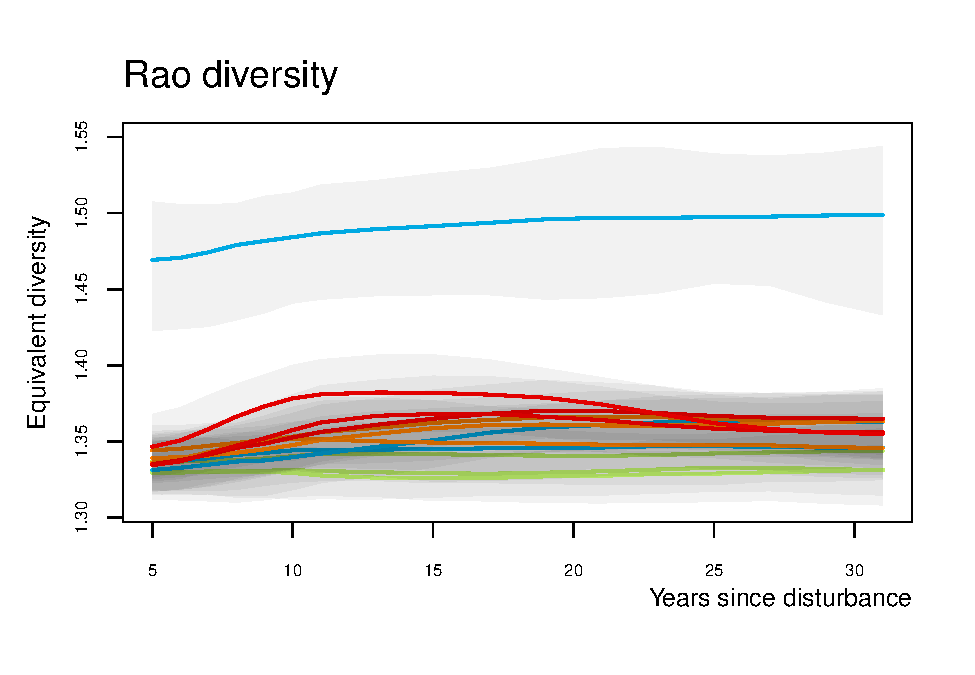
\includegraphics[width=1\linewidth]{WholePlotTrajectories_files/figure-latex/DivFun-1} 

}

\caption{Trajectories of the Rao functional diversity over 30 years after disturbance. Trajectories correspond to the median (solid line) and 0.025 and 0.975 percentile (gray envelope) observed after 50 iteration of the taxonomic uncertainty propagation. Initial treatments are represented by solid lines colorswith green for control, blue for T1,orange for T2 and red for T3.and the missing trait value filling processes.}\label{fig:DivFun}
\end{figure}

\section{Discussion}\label{discussion}

\subsection{A validation of the intermediate disturbance
hypothesis}\label{a-validation-of-the-intermediate-disturbance-hypothesis}

The monitoring 30 years of disturbed forest communities confirmed the
limited direct impact of low disturbance on species richness as it was
found for impact survey of selective logging
\citep{Cannon1998, Baraloto2012a}. Only the most disturbed plots had not
fully achieved the ongoing recovery of genus richness, although all had
already reached equivalent levels as those of some control plots. Such
long time richness recovery had already been observed in several logging
experiments, which also highlighted the role of random disturbance
damage in the richness decrease \citep{deAvila2015, Hu2018}.

The evenness of all disturbed plots and the richness of low disturbance
plots on the other hand mainly followed an asymptotic growth sharply
increasing until 15 years after disturbance. Such increased evenness is
explained by a much more homogeneous species distribution after
disturbance. Communities composition after disturbance is either due to
the old, pre-disturbance survivors or to the recruited trees. The
composition of old survivors proved to mirror the initial community
\citep{Herault2018}, the observed composition turnover would stem from
an enhanced the growth and survival of previously infrequent species
which, along with the IDH, reorganizes the typical high dominance
structure of hyperdiverse mature forests. This increase in taxonomic
diversity was accompanied by an increased taxonomic dissimilarity to
initial state along time, translating a a taxonomic turnover benefiting
to pioneers and light demanding species, as illustrated by the
communities functional shifts towards resource-acquisitive strategies
(sharp increase in the SLA, leaf thickness and bark thickness and
decrease in wood density, leaf toughness and maximum height)
\citep{Westoby1998, Wright2004, Reich2014}. Post-disturbance changes in
abiotic environment and competitive pressure then well favored pioneers
outcompeting other species when abiotic resources are abundant but
otherwise excluded in mature forests by long-lived, resistant and shade
tolerant species. The trajectories of proportions among seed mass
classes besides revealed the enhanced growth of small seeded, large
dispersive, species and therefore the importance of species reproductive
strategy which further supported the role of species dispersion and
demographic strategy for the post-disturbance dynamics, as suggested by
the IDH \citep{TerSteege2001, Flores2006, Haddad2008}.

\subsection{On the recovery of disturbed
communities}\label{on-the-recovery-of-disturbed-communities}

The functional diversity followed a hump-back trajectory which maximum
was positively correlated to the disturbance intensity
(\(\rho_{spearman}=\)) and after 30 years, all disturbed plots had
recovered diversities close to their initial values. Similar hump-back
trajectories were followed by all leaf and stem functional traits and
life history traits, to the exception of leaf chlorophyll content.
Although the return to initial values was still ongoing the recovery of
functional diversity and average communities trait values was
undeniable. This translated the recovery of ecosystems processes
\citep{Guariguata2001}, as functional traits are the most direct link
between biodiversity and ecosystem functioning \citep{Diaz2005}. Same
recovery trajectories were followed by taxonomic and functional
composition which argued for communities convergence and the maintenance
of plots initial difference
\citep{Hubbell1999, Molino2001, Baraloto2012a}. These compositon
difference, and probably also some abiotic parameters, besides strongly
determined the maximum and time path of the trajectories which, despite
an homogeneous trend were quite variable among plots.

\subsection{Functional redundancy of disturbed
ecosystems}\label{functional-redundancy-of-disturbed-ecosystems}

Despite the consistent recovery of initial diversity and composition
there was a time lag between the communities taxonomic and functional
characteristics. Taxonomic composition had longer time path and while
communities had recovered their functional diveristy, their taxonomic
composition and evenness remained higher than before disturbance. This
delay between functional and taxonomic dynamics was already observed for
grasslands \citep{Tilman1997, Mouillot2011} and more recently for
tropical forests \citep{Lohbeck2015, Guariguata2001}. Communities
functional diversity rely, according to the ``vegetation quantity
effect'' \citep{Grime1998}, on the functional strategy of dominant
species. Communities functional trajectory is then first driven by the
increase of dominant species diversity and evenness following
disturbance and then by the emergence of recruitment of species
progressively resembling the old pre-disturbance community which
decreased the diversity. Dominant species then restored the functional
diversity and the dominant functional type of the community although the
functional and taxonomic composition remained altered and the infrequent
species of initial communities are still missing to plots recovery. The
functional traits trajectories suggest that those species would match
the dominant functional type therefore increasing communities functional
redundancy. The functional overlap between species is typical of the
huge biodiversity of tropical forests \citep{Bellwood2006}, and proved
far from recovery 03 years after disturbance. It is though a determinant
of forests resilience and should be accounted for
\citep{Trenbath1999, Elmqvist2003, Diaz2005}.

Long-term alteration of functional redundancy besides came along with
persistent compositional changes which most probably impact disturbance
resistant species \citep{Haddad2008} and probably lianas or epiphytes
\citep{Martin2013}, and the modification of environmental conditions
like soils nutrient cycling and compaction \citep{Olander2005} forest
resilience remains under question \citep{Chazdon2003a}. New conditions
would not only be longer lasting but self-maintained as tied to
disturbance regime \citep{Burslem2000}. Specificaly, this would impair
species contingent to undisturbed forests, threatening their
maintenance, and run the risk to loose cornerstone species and trigger
unexpected ecological consequences
\citep{Jones1994, Diaz2005, Gardner2007}.

\section{Conclusions}\label{conclusions}

Our study showed the significant impact of disturbance on tropical
forests communities. The subsequent diversity trajectories confirmed the
intermediate disturbance hypothesis debated for tropical forests through
their correlation with disturbance intensity. Besides it revealed the
contrasting response of taxonomic and functional characteristics,
specifically the decoupling between communities taxonomic evenness and
their functional diversity and dominant functional traits values. The
long-term disturbance trajectories observed highlighted the unachieved
but consistent recovery of communities assembly for the lowest
disturbance intensity but questioned it after higher disturbance.

%----------------------------------------------------------------------------------------
%	REFERENCE LIST
%----------------------------------------------------------------------------------------

\bibliographystyle{mee}
\bibliography{references.bib}

%----------------------------------------------------------------------------------------

\end{document}
